\chapter{Measuring the Helicity Polarisation of the $\PW$ Boson}
\section{Introduction}
The study of \Wjets production at a hadron collider presents an important
opportunity for furthering understanding of the underlying Electroweak and
\ac{QCD} processes. In particular, since it is one of a relatively small number
of processes for which highly precise \ac{NLO} calculations have been performed,
experimental measurements can give a direct constraint on the \acp{PDF}. \Wjets
production is also of considerable interest in the context of \ac{NP} searches
where these events are often a dominant background. Finally, the neutrino in the
leptonic decay mode provides a source of ``real'' missing energy which can be
useful in the understanding of detector effects relevant to searches for
\acs{WIMP}-type particles present in \ac{SUSY} and other theories.

\section{Background}
Some theoretical background relating to \PW helicity effects has been presented
in Section~TODO. Here, the discussion will be oriented towards a more
experimental context.

\subsection{Polarisation Effects Parallel to the Beam Line}
For small values of \PW transverse momentum, \PtW the differential angular
cross-section for the process
$\Pp\Pp\longrightarrow\PWpm\longrightarrow\Plpm\Pgnl$ follows the Drell-Yan
distribution
\begin{equation}
\frac{dN}{d(\cos\theta)} \propto (1\mp \cos\theta)^2
\end{equation}

It is well known from straightforward helicity arguments\cite{mirkes_w_1994}that
\PW produced along the beam axis will exhibit a 100\% left-handed polarization. This
can be seen by considering the leading order partonic subprocesses
\begin{equation}
\Pup\APdown \longrightarrow \PWp \qquad\textrm{and}\qquad
\Pdown\APup\longrightarrow\PWm
\end{equation}
Firstly, note that the fraction of the proton momentum carried by the quark (as
determined by the \aclp{PDF}) is greater than that of the anti-quark. In
addition given that the \ac{LHC} is a $\Pp\Pp$ collider, valence anti-quarks are
not present. Anti-quarks must be drawn from the sea and are therefore likely to
be low momentum. Taking these two facts together, the quark is very likely to be
higher momentum than the anti-quark. By momentum conservation, it is expected
that the \PW will be produced overwhelmingly in the direction of the original
quark. Then given the \VminusA nature of the weak interaction, it is seen that
the quark must be left-handed and, by helicity conservation the \PW will be
polarised nearly 100\% left-handedly along the beam axis. A small dilution will
occur in instances where the anti-quark has by chance a larger momentum fraction
than the quark.

It is worth mentioning that the situation is not identical at the Tevatron
$\Pp\Pap$ collider. Although the \PWp also possess a 100\% left-handed
polarisation along the beamline (via similar arguments to those given above),
the \PWm are found to have a near 100\% right-handed polarisation. This is a
result of the subprocess $\APup\Pdown\longrightarrow\PWm$ where this time the
\APup carries more momentum.

\subsection{Polarisation Effects in the Transverse Plane}
In the case, where the \PW carries a significant transverse momentum \PtW, the
situation is more complex. To simplify matters, one only needs to consider the
\PWp case as the \PWm case is very similar. At leading order, three subprocesses
should be considered,
\begin{equation}
\Pup\Pgluon\longrightarrow\PWp\Pdown\;\textrm{,} \qquad
\Pup\APdown\longrightarrow\PWp\Pgluon\qquad\textrm{and} \qquad
\Pgluon\APdown\longrightarrow\PWp\APup
\label{eqn:w1jet_processes}
\end{equation}
For sufficiently large \PtW, the soft gluon enhancement of
$\Pup\APdown\longrightarrow\PWp\Pgluon$ and the quark-gluon subprocess is found
to dominate. It has been found that 70-80\% of $\PW+N$~jet ($N \leq 4$)
production at \ac{LO} is initiated by this subprocess.

Considering the quark-gluon subprocess, the $s$ and $t$ channel diagrams are
shown in Figure~\ref{fig:w1jet_st}. For the $s$ channel diagram, the on-shell
\Pdown quark is directly coupled to the \PW and therefore must be in a negative
helicity state (i.e. left-handed). Assuming a positive helicity for the W boson
(as depicted in Figure~\ref{fig:w1jet_st_s}), the spin along the $\PW\Pdown$
axis is $1+\frac{1}{2} = \frac{3}{2}$. Such a configuration is not allowed for the
\spinhalf off-shell quark and thus the $s$-channel diagram should lead to a 100\%
left-handed polarisation of the \PW. In contrast, the $t$ channel diagram is not
similarly constrained by spin arguments (since the \PW is not coupled directly
to the quark) and thus the helicity polarisation will not be seen.

It can be shown that for a left-handed incoming gluon, the $t$-channel diagram
can be made to vanish. For a right-handed gluon, the \PW polarisation is not
constrained but has been shown to become predominantly right-handed at high
\PtW. At high \PtW, the outgoing \PW helicity will be almost 100\% correlated
with the incoming gluon and due to a factor 4 difference in the size of the
corresponding matrix elements, the \PW is expected to asymptotically approach an
80\% left-handed polarisation with increasing \PtW.
\begin{figure}
\centering
\subfloat[]{\label{fig:w1jet_st_s}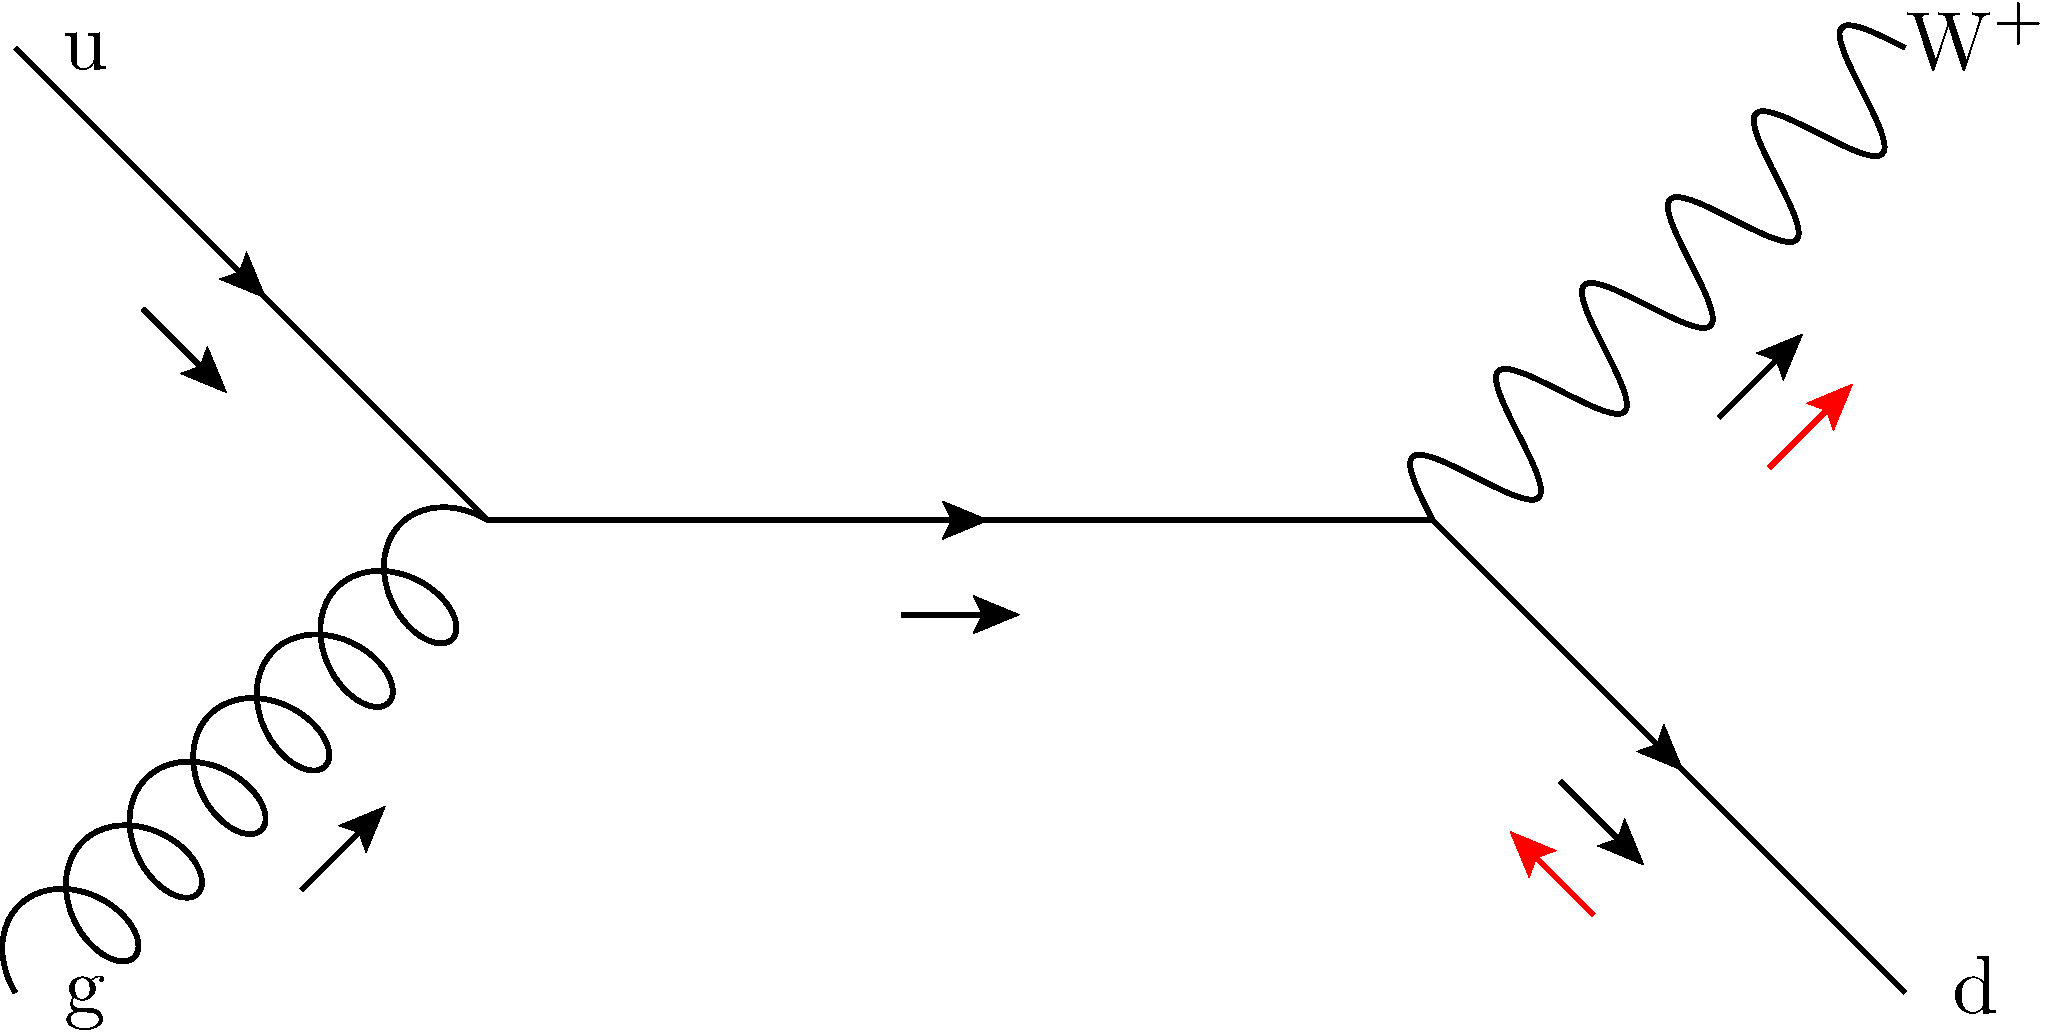
\includegraphics[width=0.5\textwidth]{fig/wpol_1jet_s}}\quad
\subfloat[]{\label{fig:w1jet_st_t}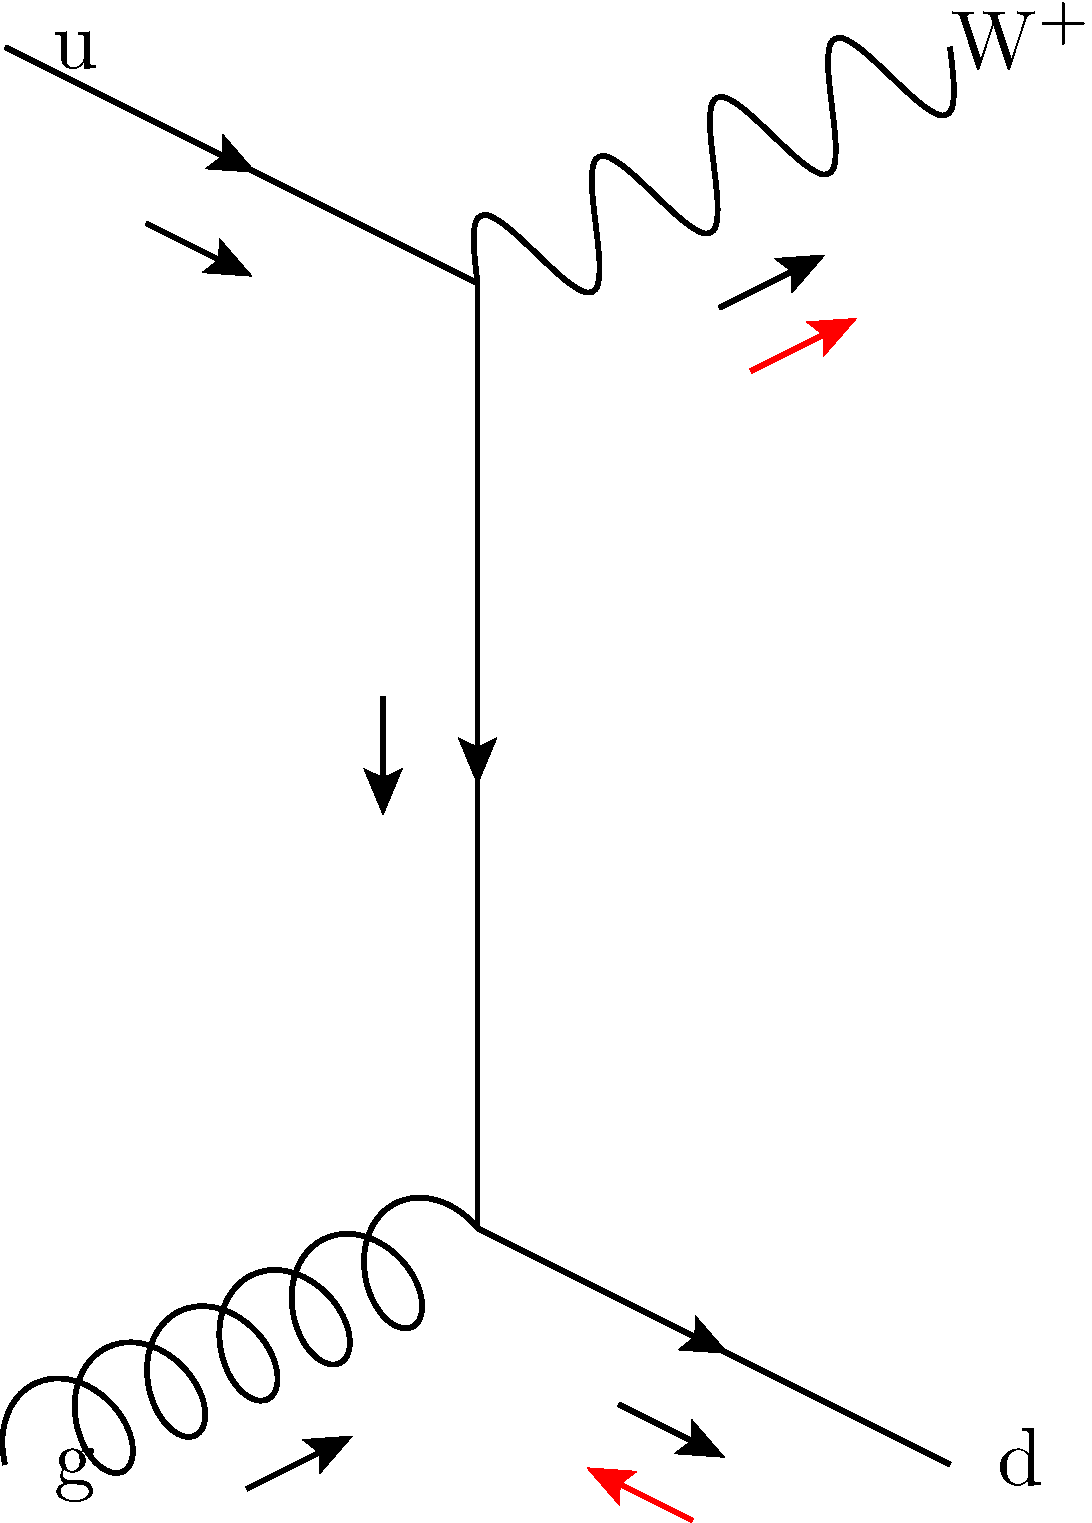
\includegraphics[width=0.25\textwidth]{fig/wpol_1jet_t}}
\caption{Diagrams showing the $\Pup\Pgluon\longrightarrow\PWp\Pdown$ subprocess
  in the \subref{fig:w1jet_st_s} $s$ and \subref{fig:w1jet_st_t} $t$ channels. The black displaced arrows indicate the particle
  momenta. For the $s$ channel diagram, the helicity vectors are shown as red
  arrows, for the case of a right-handed \PW boson.}
\label{fig:w1jet_st}
\end{figure}

Writing the amplitudes of the subprocesses in Equation~\ref{eqn:w1jet_processes}
in terms of spinor products, two distinct expressions emerge,

\begin{eqnarray*}
\mathcal{A}^{\textrm{tree}}_{(a)} &\propto&
\frac{\left<\Pdown\nu\right>^2}{\left<\Pup\Pgluon\right>\left<\Pgluon\Pdown\right>}\\
\mathcal{A}^{\textrm{tree}}_{(b)} &\propto&
\frac{\left[\Pup\Pe\right]^2}{\left[\Pup\Pgluon\right]\left[\Pgluon\Pdown\right]}
\end{eqnarray*}
where factors common to both expressions are not shown. The corresponding
cross-sections are
\begin{equation}
d\sigma^{\textrm{LO}}_{(a)} \propto (k_{\Pdown} \dot k_{\Pneutrino})^2 \quad
d\sigma^{\textrm{LO}}_{(b)} \propto (k_{\Pup} \dot k_{\Pe})^2
\label{eqn:w1jet_xs}
\end{equation}
where the $k$ are Lorentz vectors representing the particle momenta. For each
subprocess, the helicity configurations corresponding to $(a)$ and $(b)$ are
shown in the upper and lower rows of Figure~\ref{fig:w1jet_modes} respectively.

Starting with the subprocess $\Pup\Pgluon\longrightarrow\PWp\Pdown$, the $(a)$
expression in \ref{eqn:w1jet_xs} correlates the axis of the \Pdown quark with the
neutrino (see Figure~\ref{fig:w1jet_modes_1a}). Due to the \VminusA coupling, the
neutrino must have a left-handed helicity and, via angular momentum
conservation, so too the \PW. The angular dependence is
$(1-\cos\tilde{\theta}^*)^2$ where $\tilde{\theta^*}$ is the angle of the
charged decay lepton with the \PW flight direction in the centre of mass
frame. In contrast, considering an identical particle configuration but with
helicities corresponding to $(b)$ (Figure~\ref{fig:w1jet_modes_1b}), the
\Ppositron direction is now correlated with the incoming beam
direction. Boosting to the \PW rest frame, at high \PtW, the incoming quark and
gluon are nearly parallel and, given a scattering angle of 90\degrees, the \Pup
quark momentum is seen to be half that of the \Pdown quark. The angular
dependence is thus $\frac{1}{4}(1+\cos\tilde{\theta}^*)^2$ yielding a
right-handed polarisation at a quarter of the rate of the left-handed component.

For the subdominant process $\Pup\APdown\longrightarrow\PWp\Pgluon$, the terms
in Eqn~\ref{eqn:w1jet_xs} correlate the momenta of the decay leptons with the
beam direction. The two cases are shown in Figures~\ref{fig:w1jet_modes_2a} and
\ref{fig:w1jet_modes_2b}. Although it can be seen once again that a left-handed
and right-handed polarisation emerge, in this case they are found to cancel for
a scattering angle of 90\degrees and thus give no net polarisation. Lastly, for
the subprocess $\Pgluon\APdown\longrightarrow\PWp\APup$, show in
Figures~\ref{fig:w1jet_modes_3a} and \ref{fig:w1jet_modes_3b}, the $(b)$
contribution correlated the \Pup quark with the \Ppositron direction, leading to a
dominantly right-handed polarisation. However, since the \ac{PDF} $\APdown(x)$
is much smaller than $\Pup(x)$, this effect is largely washed out by the
dominant left-handed polarisation mode.

\begin{figure}
\centering
\subfloat[]{\label{fig:w1jet_modes_1a}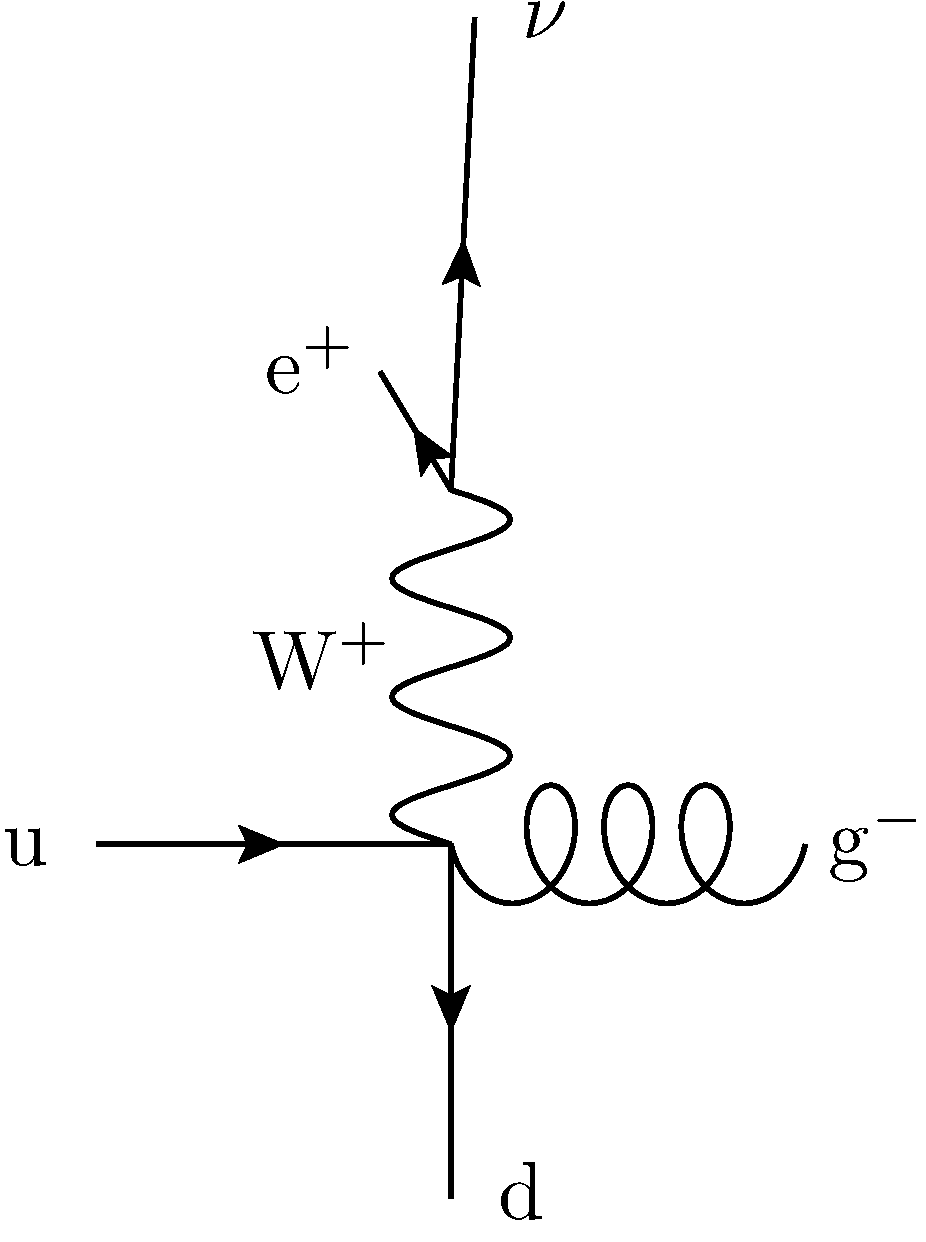
\includegraphics[width=0.3\textwidth]{fig/wpol_prod_a}}\quad
\subfloat[]{\label{fig:w1jet_modes_2a}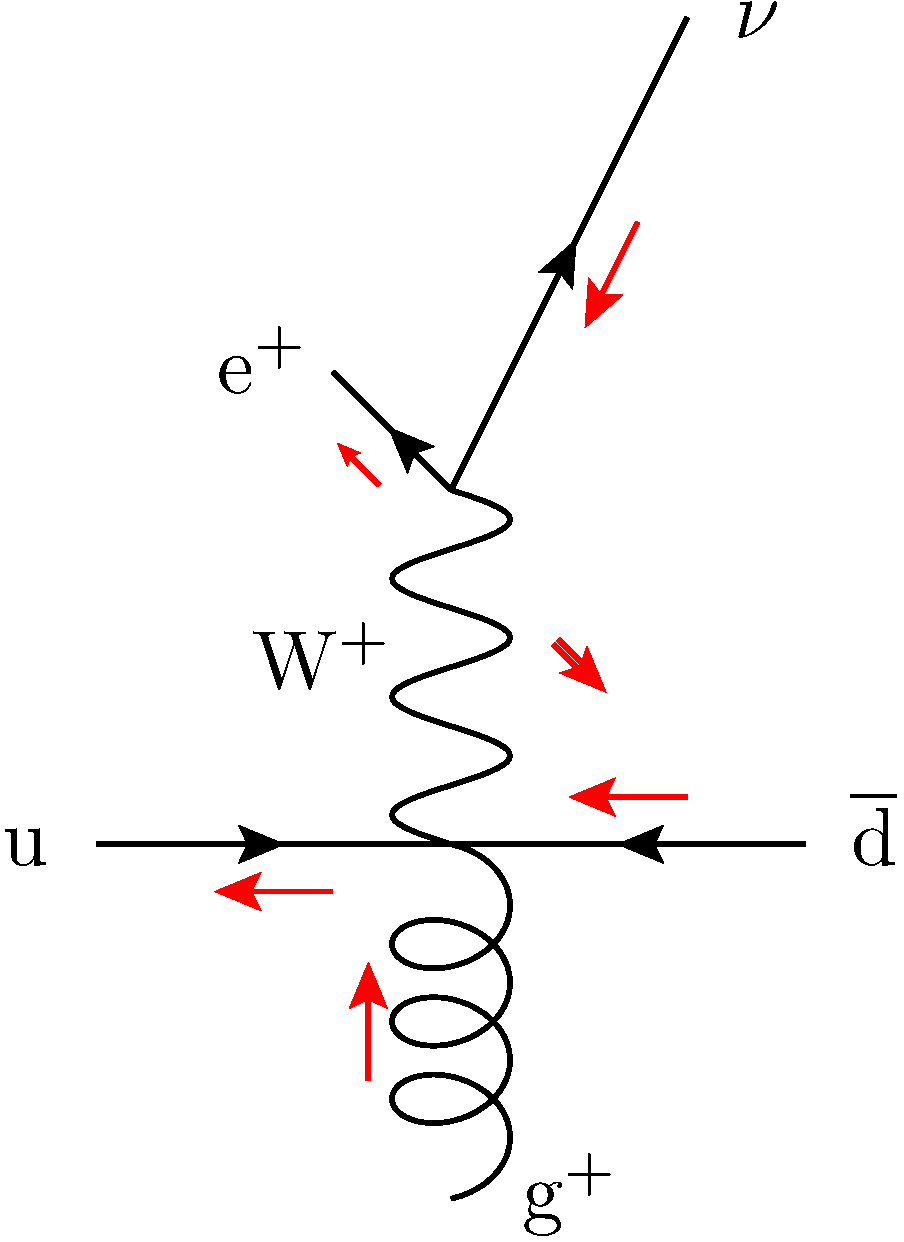
\includegraphics[width=0.3\textwidth]{fig/wpol_prod_b}}\quad
\subfloat[]{\label{fig:w1jet_modes_3a}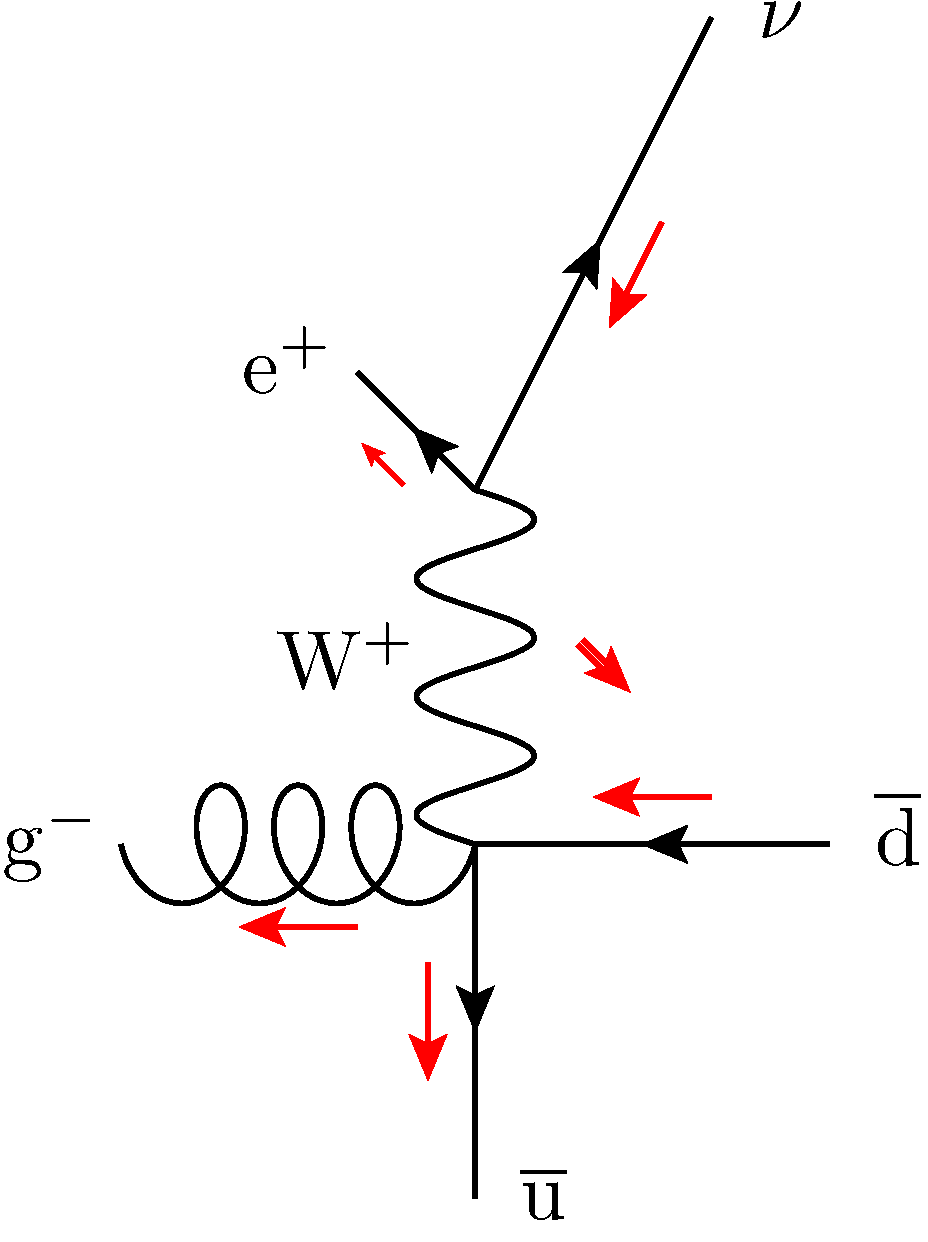
\includegraphics[width=0.3\textwidth]{fig/wpol_prod_c}}\\
\subfloat[]{\label{fig:w1jet_modes_1b}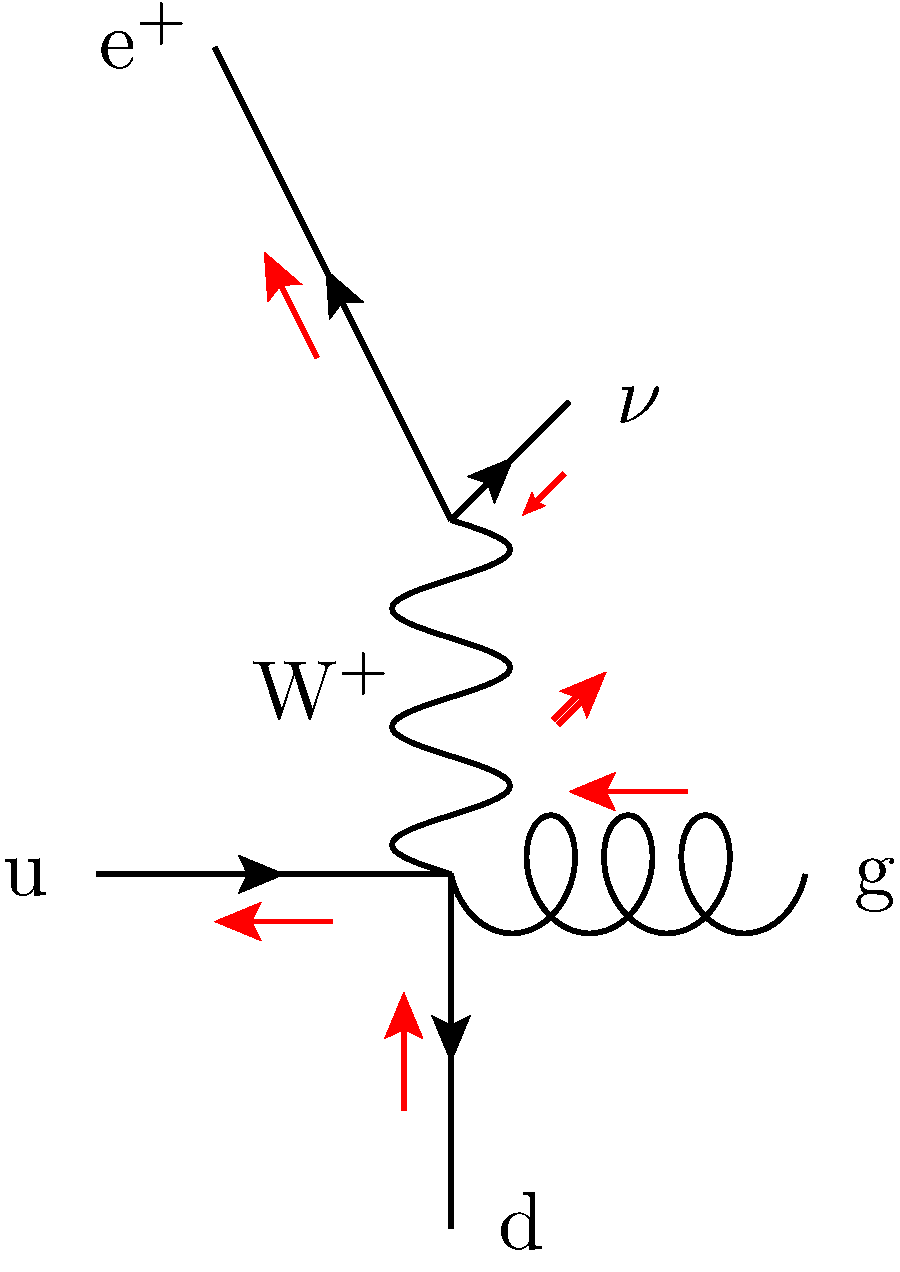
\includegraphics[width=0.3\textwidth]{fig/wpol_prod_d}}\quad
\subfloat[]{\label{fig:w1jet_modes_2b}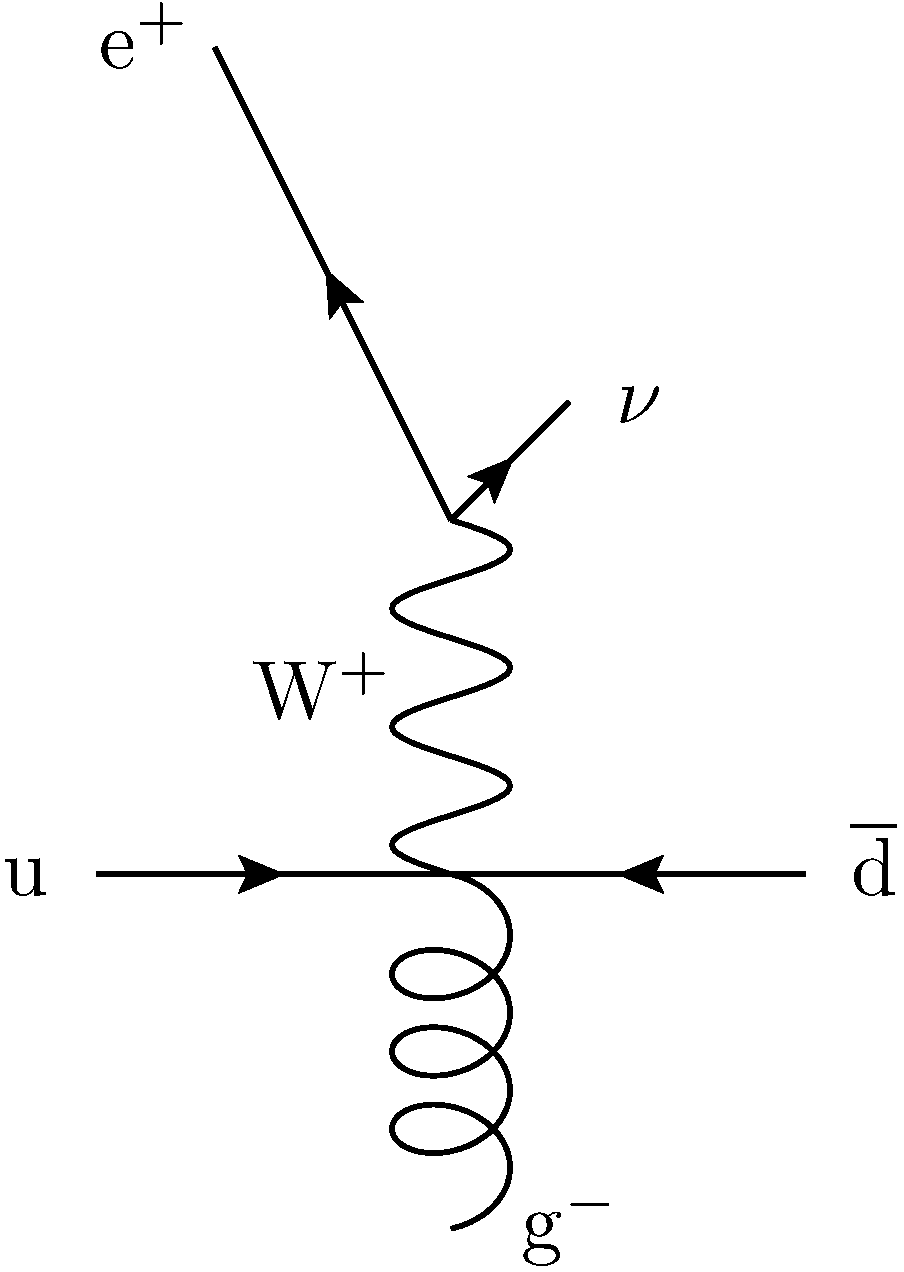
\includegraphics[width=0.3\textwidth]{fig/wpol_prod_e}}\quad
\subfloat[]{\label{fig:w1jet_modes_3b}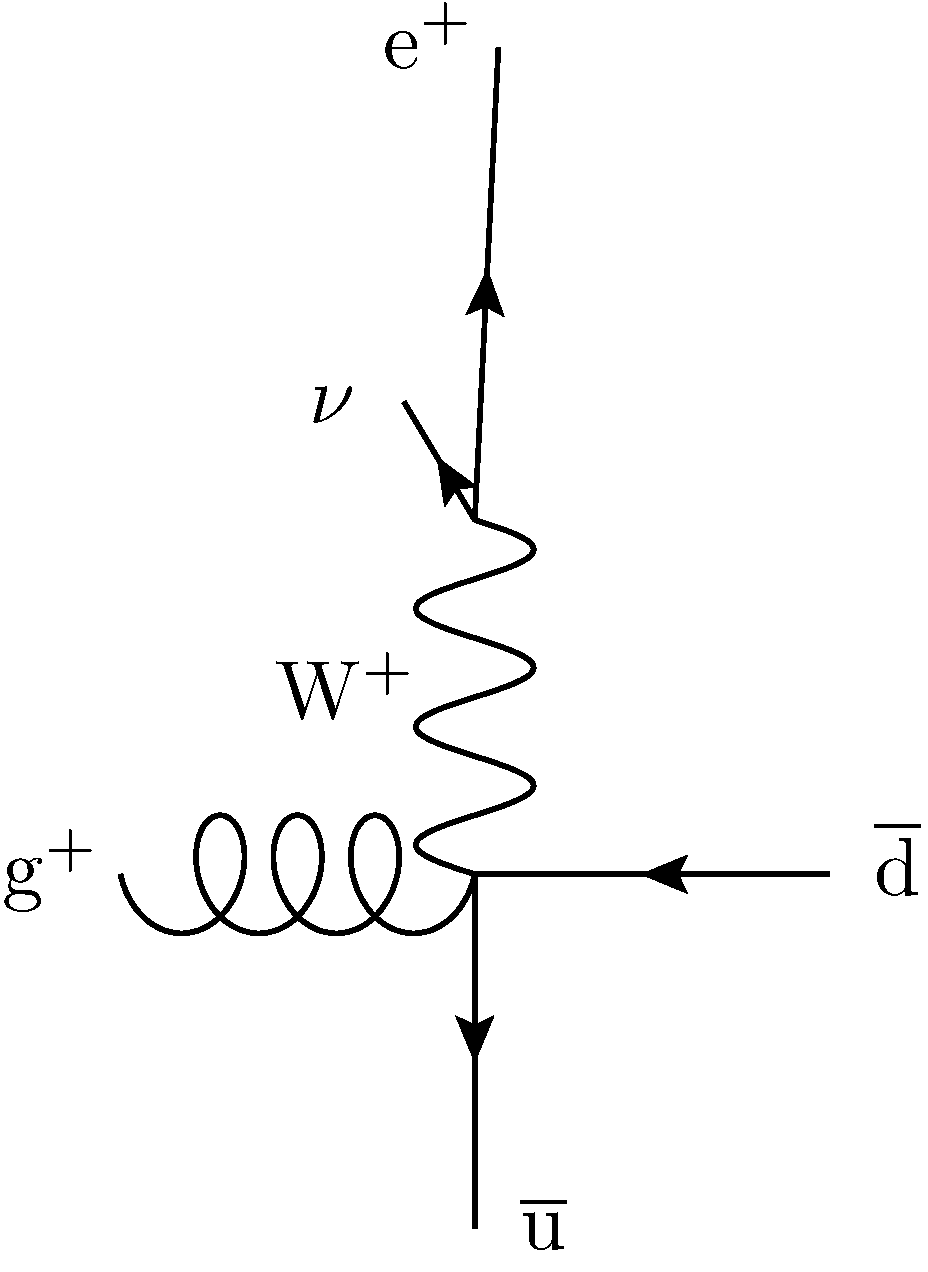
\includegraphics[width=0.3\textwidth]{fig/wpol_prod_f}}
\caption{Illustrations of $\PWplus+1$~jet production modes at the LHC. The
  gluon superscript indicates its helicity}
\label{fig:w1jet_modes}
\end{figure}
%%% Local Variables:
%%% mode: latex
%%% TeX-master: "../thesis"
%%% End:
